% Options for packages loaded elsewhere
\PassOptionsToPackage{unicode}{hyperref}
\PassOptionsToPackage{hyphens}{url}
%
\documentclass[
]{article}
\usepackage{amsmath,amssymb}
\usepackage{iftex}
\ifPDFTeX
  \usepackage[T1]{fontenc}
  \usepackage[utf8]{inputenc}
  \usepackage{textcomp} % provide euro and other symbols
\else % if luatex or xetex
  \usepackage{unicode-math} % this also loads fontspec
  \defaultfontfeatures{Scale=MatchLowercase}
  \defaultfontfeatures[\rmfamily]{Ligatures=TeX,Scale=1}
\fi
\usepackage{lmodern}
\ifPDFTeX\else
  % xetex/luatex font selection
\fi
% Use upquote if available, for straight quotes in verbatim environments
\IfFileExists{upquote.sty}{\usepackage{upquote}}{}
\IfFileExists{microtype.sty}{% use microtype if available
  \usepackage[]{microtype}
  \UseMicrotypeSet[protrusion]{basicmath} % disable protrusion for tt fonts
}{}
\makeatletter
\@ifundefined{KOMAClassName}{% if non-KOMA class
  \IfFileExists{parskip.sty}{%
    \usepackage{parskip}
  }{% else
    \setlength{\parindent}{0pt}
    \setlength{\parskip}{6pt plus 2pt minus 1pt}}
}{% if KOMA class
  \KOMAoptions{parskip=half}}
\makeatother
\usepackage{xcolor}
\usepackage[margin=1in]{geometry}
\usepackage{color}
\usepackage{fancyvrb}
\newcommand{\VerbBar}{|}
\newcommand{\VERB}{\Verb[commandchars=\\\{\}]}
\DefineVerbatimEnvironment{Highlighting}{Verbatim}{commandchars=\\\{\}}
% Add ',fontsize=\small' for more characters per line
\usepackage{framed}
\definecolor{shadecolor}{RGB}{248,248,248}
\newenvironment{Shaded}{\begin{snugshade}}{\end{snugshade}}
\newcommand{\AlertTok}[1]{\textcolor[rgb]{0.94,0.16,0.16}{#1}}
\newcommand{\AnnotationTok}[1]{\textcolor[rgb]{0.56,0.35,0.01}{\textbf{\textit{#1}}}}
\newcommand{\AttributeTok}[1]{\textcolor[rgb]{0.13,0.29,0.53}{#1}}
\newcommand{\BaseNTok}[1]{\textcolor[rgb]{0.00,0.00,0.81}{#1}}
\newcommand{\BuiltInTok}[1]{#1}
\newcommand{\CharTok}[1]{\textcolor[rgb]{0.31,0.60,0.02}{#1}}
\newcommand{\CommentTok}[1]{\textcolor[rgb]{0.56,0.35,0.01}{\textit{#1}}}
\newcommand{\CommentVarTok}[1]{\textcolor[rgb]{0.56,0.35,0.01}{\textbf{\textit{#1}}}}
\newcommand{\ConstantTok}[1]{\textcolor[rgb]{0.56,0.35,0.01}{#1}}
\newcommand{\ControlFlowTok}[1]{\textcolor[rgb]{0.13,0.29,0.53}{\textbf{#1}}}
\newcommand{\DataTypeTok}[1]{\textcolor[rgb]{0.13,0.29,0.53}{#1}}
\newcommand{\DecValTok}[1]{\textcolor[rgb]{0.00,0.00,0.81}{#1}}
\newcommand{\DocumentationTok}[1]{\textcolor[rgb]{0.56,0.35,0.01}{\textbf{\textit{#1}}}}
\newcommand{\ErrorTok}[1]{\textcolor[rgb]{0.64,0.00,0.00}{\textbf{#1}}}
\newcommand{\ExtensionTok}[1]{#1}
\newcommand{\FloatTok}[1]{\textcolor[rgb]{0.00,0.00,0.81}{#1}}
\newcommand{\FunctionTok}[1]{\textcolor[rgb]{0.13,0.29,0.53}{\textbf{#1}}}
\newcommand{\ImportTok}[1]{#1}
\newcommand{\InformationTok}[1]{\textcolor[rgb]{0.56,0.35,0.01}{\textbf{\textit{#1}}}}
\newcommand{\KeywordTok}[1]{\textcolor[rgb]{0.13,0.29,0.53}{\textbf{#1}}}
\newcommand{\NormalTok}[1]{#1}
\newcommand{\OperatorTok}[1]{\textcolor[rgb]{0.81,0.36,0.00}{\textbf{#1}}}
\newcommand{\OtherTok}[1]{\textcolor[rgb]{0.56,0.35,0.01}{#1}}
\newcommand{\PreprocessorTok}[1]{\textcolor[rgb]{0.56,0.35,0.01}{\textit{#1}}}
\newcommand{\RegionMarkerTok}[1]{#1}
\newcommand{\SpecialCharTok}[1]{\textcolor[rgb]{0.81,0.36,0.00}{\textbf{#1}}}
\newcommand{\SpecialStringTok}[1]{\textcolor[rgb]{0.31,0.60,0.02}{#1}}
\newcommand{\StringTok}[1]{\textcolor[rgb]{0.31,0.60,0.02}{#1}}
\newcommand{\VariableTok}[1]{\textcolor[rgb]{0.00,0.00,0.00}{#1}}
\newcommand{\VerbatimStringTok}[1]{\textcolor[rgb]{0.31,0.60,0.02}{#1}}
\newcommand{\WarningTok}[1]{\textcolor[rgb]{0.56,0.35,0.01}{\textbf{\textit{#1}}}}
\usepackage{longtable,booktabs,array}
\usepackage{calc} % for calculating minipage widths
% Correct order of tables after \paragraph or \subparagraph
\usepackage{etoolbox}
\makeatletter
\patchcmd\longtable{\par}{\if@noskipsec\mbox{}\fi\par}{}{}
\makeatother
% Allow footnotes in longtable head/foot
\IfFileExists{footnotehyper.sty}{\usepackage{footnotehyper}}{\usepackage{footnote}}
\makesavenoteenv{longtable}
\usepackage{graphicx}
\makeatletter
\def\maxwidth{\ifdim\Gin@nat@width>\linewidth\linewidth\else\Gin@nat@width\fi}
\def\maxheight{\ifdim\Gin@nat@height>\textheight\textheight\else\Gin@nat@height\fi}
\makeatother
% Scale images if necessary, so that they will not overflow the page
% margins by default, and it is still possible to overwrite the defaults
% using explicit options in \includegraphics[width, height, ...]{}
\setkeys{Gin}{width=\maxwidth,height=\maxheight,keepaspectratio}
% Set default figure placement to htbp
\makeatletter
\def\fps@figure{htbp}
\makeatother
\setlength{\emergencystretch}{3em} % prevent overfull lines
\providecommand{\tightlist}{%
  \setlength{\itemsep}{0pt}\setlength{\parskip}{0pt}}
\setcounter{secnumdepth}{-\maxdimen} % remove section numbering
\ifLuaTeX
  \usepackage{selnolig}  % disable illegal ligatures
\fi
\IfFileExists{bookmark.sty}{\usepackage{bookmark}}{\usepackage{hyperref}}
\IfFileExists{xurl.sty}{\usepackage{xurl}}{} % add URL line breaks if available
\urlstyle{same}
\hypersetup{
  pdftitle={Aula-04},
  pdfauthor={Panosso AR},
  hidelinks,
  pdfcreator={LaTeX via pandoc}}

\title{Aula-04}
\author{Panosso AR}
\date{2023-12-07}

\begin{document}
\maketitle

\hypertarget{relatuxf3rio-aula-4}{%
\section{Relatório Aula 4}\label{relatuxf3rio-aula-4}}

Nesta aula, foram apresentados os conceitos de visualização de dados, e
modelagem a partir dos pacotes ggplot e corrplot. Em adição, foram
estudados:

\begin{itemize}
\item
  Estrutura de repetição;
\item
  Teste de normalidade;
\item
  Construção de relatórios
\end{itemize}

\hypertarget{marcauxe7uxf5es-de-texto}{%
\subsection{Marcações de texto}\label{marcauxe7uxf5es-de-texto}}

Subscrito: CO\textsubscript{2} =
\texttt{CO\textasciitilde{}2\textasciitilde{}}

Negrito: palavra \textbf{em negrito} = \texttt{palavra\ **em\ negrito**}

Itálico: palavra \emph{em itálico} = \texttt{palavra\ *em\ itálico*}

\hypertarget{adicionando-uma-imagem}{%
\subsection{Adicionando uma imagem}\label{adicionando-uma-imagem}}

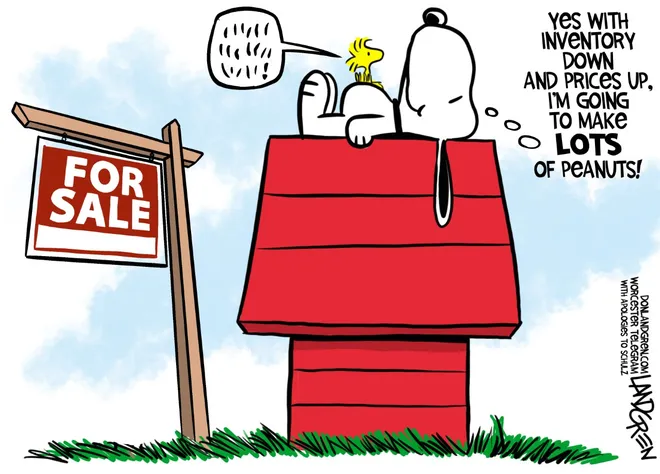
\includegraphics{snoopy.png}

FONTE:
\href{https://www.telegram.com/story/opinion/2021/04/23/peanuts-snoopy-cartoon-don-landgren/7332261002/}{LINK}

\hypertarget{adiuxe7uxe3o-de-vuxeddeos-utilize-o-cuxf3digo-de-incorporauxe7uxe3o}{%
\subsection{Adição de vídeos, utilize o código de
incorporação}\label{adiuxe7uxe3o-de-vuxeddeos-utilize-o-cuxf3digo-de-incorporauxe7uxe3o}}

\hypertarget{criauxe7uxe3o-de-um-modelo-matemuxe1tico}{%
\subsection{Criação de Um modelo
matemático}\label{criauxe7uxe3o-de-um-modelo-matemuxe1tico}}

Modelo fatorial de dois fatores

\[
y_{ij} = \mu+\alpha_i+\beta_j+(\alpha \beta)_{ij} + \epsilon_{ij}
\]

Função densidade normal

\[
f(x)=\frac{1}{\sqrt{2\pi\sigma^2}} e^{-\frac{1}{2}\frac{(x-\mu)^2}{\sigma^2} }
\] \#\# Criação de Tabela

\begin{longtable}[]{@{}lcccr@{}}
\toprule\noalign{}
Tratamento & Rep.1 & Rep.2 & Rep.3 & Total \\
\midrule\noalign{}
\endhead
\bottomrule\noalign{}
\endlastfoot
T1 & 4 & 5 & 3 & 12 \\
T2 & 8 & 7 & 10 & 25 \\
T3 & 9 & 4 & 12 & 25 \\
\end{longtable}

\hypertarget{trechos-de-cuxf3digos-do-r-chunk.}{%
\subsection{Trechos de códigos do R
(Chunk).}\label{trechos-de-cuxf3digos-do-r-chunk.}}

Para gerar um trecho de código use o comando

\textbf{Control + Alt + i}

\hypertarget{carregando-os-pacotes}{%
\subsubsection{Carregando os pacotes}\label{carregando-os-pacotes}}

\begin{Shaded}
\begin{Highlighting}[]
\FunctionTok{library}\NormalTok{(tidyverse)}
\FunctionTok{library}\NormalTok{(readxl)}
\end{Highlighting}
\end{Shaded}

\hypertarget{lendo-o-arquivo-geomorfologia}{%
\subsubsection{Lendo o arquivo
geomorfologia}\label{lendo-o-arquivo-geomorfologia}}

\begin{Shaded}
\begin{Highlighting}[]
\NormalTok{geomorfologia }\OtherTok{\textless{}{-}} \FunctionTok{read\_rds}\NormalTok{(}\StringTok{"../data/geomorfologia.rds"}\NormalTok{)}
\end{Highlighting}
\end{Shaded}

\hypertarget{resumo-do-banco-de-dados}{%
\subsubsection{Resumo do banco de
dados}\label{resumo-do-banco-de-dados}}

\begin{Shaded}
\begin{Highlighting}[]
\NormalTok{skimr}\SpecialCharTok{::}\FunctionTok{skim}\NormalTok{(geomorfologia)}
\end{Highlighting}
\end{Shaded}

\begin{longtable}[]{@{}ll@{}}
\caption{Data summary}\tabularnewline
\toprule\noalign{}
\endfirsthead
\endhead
\bottomrule\noalign{}
\endlastfoot
Name & geomorfologia \\
Number of rows & 106 \\
Number of columns & 22 \\
\_\_\_\_\_\_\_\_\_\_\_\_\_\_\_\_\_\_\_\_\_\_\_ & \\
Column type frequency: & \\
character & 2 \\
numeric & 20 \\
\_\_\_\_\_\_\_\_\_\_\_\_\_\_\_\_\_\_\_\_\_\_\_\_ & \\
Group variables & None \\
\end{longtable}

\textbf{Variable type: character}

\begin{longtable}[]{@{}
  >{\raggedright\arraybackslash}p{(\columnwidth - 14\tabcolsep) * \real{0.1944}}
  >{\raggedleft\arraybackslash}p{(\columnwidth - 14\tabcolsep) * \real{0.1389}}
  >{\raggedleft\arraybackslash}p{(\columnwidth - 14\tabcolsep) * \real{0.1944}}
  >{\raggedleft\arraybackslash}p{(\columnwidth - 14\tabcolsep) * \real{0.0556}}
  >{\raggedleft\arraybackslash}p{(\columnwidth - 14\tabcolsep) * \real{0.0556}}
  >{\raggedleft\arraybackslash}p{(\columnwidth - 14\tabcolsep) * \real{0.0833}}
  >{\raggedleft\arraybackslash}p{(\columnwidth - 14\tabcolsep) * \real{0.1250}}
  >{\raggedleft\arraybackslash}p{(\columnwidth - 14\tabcolsep) * \real{0.1528}}@{}}
\toprule\noalign{}
\begin{minipage}[b]{\linewidth}\raggedright
skim\_variable
\end{minipage} & \begin{minipage}[b]{\linewidth}\raggedleft
n\_missing
\end{minipage} & \begin{minipage}[b]{\linewidth}\raggedleft
complete\_rate
\end{minipage} & \begin{minipage}[b]{\linewidth}\raggedleft
min
\end{minipage} & \begin{minipage}[b]{\linewidth}\raggedleft
max
\end{minipage} & \begin{minipage}[b]{\linewidth}\raggedleft
empty
\end{minipage} & \begin{minipage}[b]{\linewidth}\raggedleft
n\_unique
\end{minipage} & \begin{minipage}[b]{\linewidth}\raggedleft
whitespace
\end{minipage} \\
\midrule\noalign{}
\endhead
\bottomrule\noalign{}
\endlastfoot
sup & 0 & 1 & 1 & 3 & 0 & 3 & 0 \\
solo & 0 & 1 & 1 & 3 & 0 & 8 & 0 \\
\end{longtable}

\textbf{Variable type: numeric}

\begin{longtable}[]{@{}
  >{\raggedright\arraybackslash}p{(\columnwidth - 20\tabcolsep) * \real{0.1069}}
  >{\raggedleft\arraybackslash}p{(\columnwidth - 20\tabcolsep) * \real{0.0763}}
  >{\raggedleft\arraybackslash}p{(\columnwidth - 20\tabcolsep) * \real{0.1069}}
  >{\raggedleft\arraybackslash}p{(\columnwidth - 20\tabcolsep) * \real{0.0611}}
  >{\raggedleft\arraybackslash}p{(\columnwidth - 20\tabcolsep) * \real{0.0534}}
  >{\raggedleft\arraybackslash}p{(\columnwidth - 20\tabcolsep) * \real{0.0458}}
  >{\raggedleft\arraybackslash}p{(\columnwidth - 20\tabcolsep) * \real{0.0534}}
  >{\raggedleft\arraybackslash}p{(\columnwidth - 20\tabcolsep) * \real{0.0611}}
  >{\raggedleft\arraybackslash}p{(\columnwidth - 20\tabcolsep) * \real{0.0611}}
  >{\raggedleft\arraybackslash}p{(\columnwidth - 20\tabcolsep) * \real{0.0611}}
  >{\raggedright\arraybackslash}p{(\columnwidth - 20\tabcolsep) * \real{0.3130}}@{}}
\toprule\noalign{}
\begin{minipage}[b]{\linewidth}\raggedright
skim\_variable
\end{minipage} & \begin{minipage}[b]{\linewidth}\raggedleft
n\_missing
\end{minipage} & \begin{minipage}[b]{\linewidth}\raggedleft
complete\_rate
\end{minipage} & \begin{minipage}[b]{\linewidth}\raggedleft
mean
\end{minipage} & \begin{minipage}[b]{\linewidth}\raggedleft
sd
\end{minipage} & \begin{minipage}[b]{\linewidth}\raggedleft
p0
\end{minipage} & \begin{minipage}[b]{\linewidth}\raggedleft
p25
\end{minipage} & \begin{minipage}[b]{\linewidth}\raggedleft
p50
\end{minipage} & \begin{minipage}[b]{\linewidth}\raggedleft
p75
\end{minipage} & \begin{minipage}[b]{\linewidth}\raggedleft
p100
\end{minipage} & \begin{minipage}[b]{\linewidth}\raggedright
hist
\end{minipage} \\
\midrule\noalign{}
\endhead
\bottomrule\noalign{}
\endlastfoot
amostra & 0 & 1 & 53.50 & 30.74 & 1.00 & 27.25 & 53.50 & 79.75 & 106.00
& ▇▇▇▇▇ \\
x & 0 & 1 & 1312.50 & 768.59 & 0.00 & 656.25 & 1312.50 & 1968.75 &
2625.00 & ▇▇▇▇▇ \\
amg & 0 & 1 & 0.36 & 0.28 & 0.00 & 0.20 & 0.30 & 0.50 & 1.30 & ▇▇▂▁▁ \\
ag & 0 & 1 & 6.85 & 3.80 & 1.24 & 4.12 & 5.92 & 8.45 & 21.60 & ▇▆▂▁▁ \\
am & 0 & 1 & 28.42 & 7.61 & 13.20 & 22.80 & 28.15 & 33.32 & 48.70 &
▃▇▇▅▁ \\
af & 0 & 1 & 19.33 & 5.83 & 0.60 & 15.93 & 19.10 & 23.30 & 34.20 &
▁▂▇▆▁ \\
amf & 0 & 1 & 27.67 & 11.56 & 8.30 & 20.22 & 24.95 & 33.33 & 62.80 &
▃▇▃▂▁ \\
silte & 0 & 1 & 2.62 & 2.29 & 0.10 & 1.20 & 2.00 & 3.20 & 11.40 &
▇▅▁▁▁ \\
argila & 0 & 1 & 14.60 & 6.16 & 4.30 & 8.80 & 14.15 & 20.50 & 26.60 &
▆▆▃▇▂ \\
silte\_argila & 0 & 1 & 0.23 & 0.22 & 0.01 & 0.07 & 0.15 & 0.32 & 0.90 &
▇▂▂▁▁ \\
af\_ag & 0 & 1 & 3.99 & 3.39 & 0.14 & 1.81 & 2.91 & 5.41 & 25.40 &
▇▂▁▁▁ \\
p\_resina & 0 & 1 & 26.81 & 38.56 & 2.00 & 4.00 & 10.00 & 31.50 & 209.00
& ▇▁▁▁▁ \\
ph & 0 & 1 & 4.98 & 0.70 & 3.80 & 4.50 & 4.95 & 5.50 & 6.30 & ▆▇▇▅▅ \\
k & 0 & 1 & 0.13 & 0.08 & 0.01 & 0.08 & 0.12 & 0.17 & 0.37 & ▆▇▃▂▁ \\
ca & 0 & 1 & 3.78 & 5.52 & 0.20 & 1.40 & 2.20 & 3.20 & 27.60 & ▇▁▁▁▁ \\
mg & 0 & 1 & 0.87 & 0.82 & 0.10 & 0.40 & 0.70 & 1.00 & 3.60 & ▇▃▁▁▁ \\
h\_al & 0 & 1 & 3.03 & 1.57 & 0.60 & 1.52 & 2.80 & 4.20 & 6.40 &
▇▇▅▆▂ \\
sb & 0 & 1 & 4.78 & 6.30 & 0.31 & 1.86 & 2.92 & 4.22 & 31.30 & ▇▁▁▁▁ \\
ctc & 0 & 1 & 7.84 & 6.17 & 3.77 & 4.97 & 5.99 & 6.99 & 32.60 & ▇▁▁▁▁ \\
v & 0 & 1 & 52.68 & 25.51 & 5.00 & 35.25 & 55.00 & 73.75 & 96.00 &
▅▃▇▇▅ \\
\end{longtable}

\hypertarget{criando-um-histograma-de-argila}{%
\subsubsection{Criando um histograma de
argila}\label{criando-um-histograma-de-argila}}

\begin{Shaded}
\begin{Highlighting}[]
\NormalTok{geomorfologia }\SpecialCharTok{\%\textgreater{}\%} 
  \FunctionTok{ggplot}\NormalTok{(}\FunctionTok{aes}\NormalTok{(}\AttributeTok{x=}\NormalTok{argila, }\AttributeTok{y=}\NormalTok{..density..)) }\SpecialCharTok{+}
  \FunctionTok{geom\_histogram}\NormalTok{(}\AttributeTok{bins=}\DecValTok{10}\NormalTok{,}\AttributeTok{color=}\StringTok{"black"}\NormalTok{,}\AttributeTok{fill=}\StringTok{"gray"}\NormalTok{)}\SpecialCharTok{+}
  \FunctionTok{theme\_bw}\NormalTok{()}
\end{Highlighting}
\end{Shaded}

\includegraphics{aula-04_files/figure-latex/unnamed-chunk-4-1.pdf}

\end{document}
